% Options for packages loaded elsewhere
\PassOptionsToPackage{unicode}{hyperref}
\PassOptionsToPackage{hyphens}{url}
\PassOptionsToPackage{dvipsnames,svgnames,x11names}{xcolor}
%
\documentclass[
  10pt,
]{article}
\usepackage{amsmath,amssymb}
\usepackage{iftex}
\ifPDFTeX
  \usepackage[T1]{fontenc}
  \usepackage[utf8]{inputenc}
  \usepackage{textcomp} % provide euro and other symbols
\else % if luatex or xetex
  \usepackage{unicode-math} % this also loads fontspec
  \defaultfontfeatures{Scale=MatchLowercase}
  \defaultfontfeatures[\rmfamily]{Ligatures=TeX,Scale=1}
\fi
\usepackage{lmodern}
\ifPDFTeX\else
  % xetex/luatex font selection
\fi
% Use upquote if available, for straight quotes in verbatim environments
\IfFileExists{upquote.sty}{\usepackage{upquote}}{}
\IfFileExists{microtype.sty}{% use microtype if available
  \usepackage[]{microtype}
  \UseMicrotypeSet[protrusion]{basicmath} % disable protrusion for tt fonts
}{}
\makeatletter
\@ifundefined{KOMAClassName}{% if non-KOMA class
  \IfFileExists{parskip.sty}{%
    \usepackage{parskip}
  }{% else
    \setlength{\parindent}{0pt}
    \setlength{\parskip}{6pt plus 2pt minus 1pt}}
}{% if KOMA class
  \KOMAoptions{parskip=half}}
\makeatother
\usepackage{xcolor}
\usepackage[margin=0.72in]{geometry}
\usepackage{graphicx}
\makeatletter
\def\maxwidth{\ifdim\Gin@nat@width>\linewidth\linewidth\else\Gin@nat@width\fi}
\def\maxheight{\ifdim\Gin@nat@height>\textheight\textheight\else\Gin@nat@height\fi}
\makeatother
% Scale images if necessary, so that they will not overflow the page
% margins by default, and it is still possible to overwrite the defaults
% using explicit options in \includegraphics[width, height, ...]{}
\setkeys{Gin}{width=\maxwidth,height=\maxheight,keepaspectratio}
% Set default figure placement to htbp
\makeatletter
\def\fps@figure{htbp}
\makeatother
\setlength{\emergencystretch}{3em} % prevent overfull lines
\providecommand{\tightlist}{%
  \setlength{\itemsep}{0pt}\setlength{\parskip}{0pt}}
\setcounter{secnumdepth}{-\maxdimen} % remove section numbering
\usepackage{amsmath,amssymb,mathtools}
\usepackage{booktabs,longtable,array}
\usepackage{graphicx,float}
\graphicspath{{/mnt/data/}}
\usepackage{xcolor}
\usepackage{microtype}
\setlength{\parindent}{0pt}
\setlength{\parskip}{5pt plus 1pt minus 1pt}
\renewcommand{\arraystretch}{1.14}
\ifLuaTeX
  \usepackage{selnolig}  % disable illegal ligatures
\fi
\usepackage{bookmark}
\IfFileExists{xurl.sty}{\usepackage{xurl}}{} % add URL line breaks if available
\urlstyle{same}
\hypersetup{
  pdftitle={Chronometric Emergence Project Checkpoint},
  pdfauthor={Chronometric Emergence Project},
  colorlinks=true,
  linkcolor={blue},
  filecolor={Maroon},
  citecolor={Blue},
  urlcolor={blue},
  pdfcreator={LaTeX via pandoc}}

\title{Chronometric Emergence Project Checkpoint}
\usepackage{etoolbox}
\makeatletter
\providecommand{\subtitle}[1]{% add subtitle to \maketitle
  \apptocmd{\@title}{\par {\large #1 \par}}{}{}
}
\makeatother
\subtitle{Scientific value, novelty boundary, publication strategy, and
status after v1.6}
\author{Chronometric Emergence Project}
\date{21 August 2026}

\begin{document}
\maketitle

{
\hypersetup{linkcolor=}
\setcounter{tocdepth}{3}
\tableofcontents
}
\section{Executive assessment}\label{executive-assessment}

\subsection{Direct verdict}\label{direct-verdict}

The work is \textbf{scientifically meaningful}. It has generated a
coherent, falsifiable programme and, equally importantly, has killed
several attractive but wrong formulations.

The work is \textbf{potentially important}, but its importance is not
established. The project has not derived time, spacetime, or gravity
from first principles. Its strongest defensible thesis is narrower:

\[
\boxed{
\text{causal structure may be primitive, while proper-duration calibration can be a field-generated spectral relation.}
}
\]

There is material worth sharing and publishing, but not as one grand
paper titled ``time emerges from photons.'' The project should now be
split into focused papers with sharply bounded claims.

The current novelty verdict is:

\[
\boxed{
\text{individual ingredients are mostly established; the integrated formalism and several model-specific relations are candidate new contributions.}
}
\]

No priority claim is secure until an independent specialist literature
audit, independent derivation, and external technical review are
complete.

\section{What the project has actually
accomplished}\label{what-the-project-has-actually-accomplished}

\subsection{It found and abandoned the wrong starting
point}\label{it-found-and-abandoned-the-wrong-starting-point}

The initial photon-perspective intuition correctly exposed the absence
of proper time along a null path, but a photon has no timelike observer
frame. The first exact-null field theory also failed: its transverse
quadratic principal symbol was rank deficient in \(3+1\) dimensions.
That failure was not cosmetic. It forced the project to separate null
kinematics from the dynamics that generate scale.

The replacement soft-null two-phase EFT has a positive quadratic
Hamiltonian and real subluminal modes in its declared regime. This is a
genuine improvement over the original construction, not merely a change
in rhetoric.

\subsection{It produced a precise operational criterion for metric
time}\label{it-produced-a-precise-operational-criterion-for-metric-time}

Let clock transition \(A\) have positive local frequency \(\omega_A(x)\)
of Weyl weight \(-1\). One conformal representative calibrates every
clock if and only if

\[
\boxed{
\omega_A(x)=c_A\chi(x)
\quad\text{for all }A,
}
\]

where \(c_A\) is constant and \(\chi\) is one shared local scale field.
Equivalently,

\[
\boxed{
\mathcal S_{AB}
\equiv d\ln\frac{\omega_A}{\omega_B}=0
\quad\text{for every clock pair.}
}
\]

The one-forms \(\mathcal S_{AB}\) were named \textbf{chronometric
shear}. They are Weyl invariant: changing conformal frame cannot remove
a real differential drift between clocks.

The associated clock-space result is

\[
\boxed{
\operatorname{rank}
\left[\delta\ln(\omega_A/\omega_B)\right]
\le r,
}
\]

when the spectra depend on \(r\) independent non-universal fields. One
mismatch scalar predicts a rank-one clock network; universal chronometry
is rank zero.

The theorem is elementary once written down. Its possible value lies in
the operational interpretation, quotient-space formulation, rank test,
and connection to clock and equivalence-principle data. The
clock-hypothesis, EPS, Weyl-geometry, and chronogeometry literatures are
substantial, so this must be positioned as a refinement and synthesis,
not an invention of physical chronogeometry.

\subsection{It turned the scale problem into a concrete particle-physics
problem}\label{it-turned-the-scale-problem-into-a-concrete-particle-physics-problem}

The ordinary Standard Model Higgs is not sufficient as the sole
universal scale because real clocks also depend on QCD, nuclear
structure, dimensionless couplings, and the gravitational scale. The
project therefore introduced a deeper field \(\chi\) and attempted to
lock

\[
\frac{h}{\chi},
\qquad
\frac{\Lambda_{\mathrm{QCD}}}{\chi},
\qquad
\frac{M_{\mathrm P}}{\chi}
\]

to constants.

A conventional two-derivative hidden gauge/scalar model provides a
healthy EFT proof of principle. The optional Turok-36 interpretation
remains only an ultraviolet hypothesis because the required Lorentzian
unitarity and positive physical spectral density are unsettled.

\subsection{It found a calculable non-universal
defect}\label{it-found-a-calculable-non-universal-defect}

The QCD threshold recursion gives, for one extra colour-fundamental
Dirac fermion,

\[
\boxed{
d\ln\frac{\Lambda_3}{\chi}
=
\frac{2}{27}\,\varepsilon_\Psi\,d\theta
+\text{controlled corrections}.
}
\]

The coefficient \(2/27\) is established QCD decoupling physics. The
project-specific move is to interpret it as the transmission coefficient
from a microscopic failure of universal scale locking to observable
clock disagreement.

This leads to two falsifiable structures:

\begin{enumerate}
\def\labelenumi{\arabic{enumi}.}
\tightlist
\item
  a rank-one pattern across dissimilar clocks;
\item
  a clock/free-fall consistency relation of the form
\end{enumerate}

\[
\boxed{
\frac{\beta_{AB}}{\eta_{CD}}
=
-\frac{\Delta K_{AB}}
{\Delta Q_{\widehat m}^{\prime\,CD}}
}
\]

under the stated one-field, long-range, unscreened, QCD-dominated
assumptions.

That is more publishable than the philosophical slogan because it can be
wrong in a measurable way.

\subsection{It solved the radiative naturalness problem
conditionally}\label{it-solved-the-radiative-naturalness-problem-conditionally}

A cyclic \(Z_6\) orbit preserves an \(O(\epsilon)\) visible QCD response
while suppressing the vacuum mass to \(O(\epsilon^6)\):

\[
\boxed{
m_a^2
=
\frac{27}{320\pi^2}
\frac{M^4}{f_a^2}\epsilon^6+
O(\epsilon^7),
}
\]

\[
\boxed{
d_g
=
\frac{2}{27}
\frac{M_{\mathrm P}}{f_a}\epsilon
+
O(\alpha_s\epsilon,\epsilon^2).
}
\]

The general discrete-Goldstone mechanism is established. The candidate
contribution is the specific combination of a real vectorlike QCD
threshold, the \(2/27\) chronometric transmission, clock/free-fall
observables, and state-selected cosmology.

The condition is severe: the microscopic \(Z_6\) and continuous-shift
spurion structure must be exact enough that lower harmonics are not
reintroduced. A Wilson-line or collective-pNGB UV completion is
therefore not optional decoration; it is part of the model's
credibility.

\subsection{It tested environment, cosmology, reheating, and transport
rather than assuming them
away}\label{it-tested-environment-cosmology-reheating-and-transport-rather-than-assuming-them-away}

The environmental analysis found that Earth, the Sun, and laboratory
sources do not thin-shell screen the benchmark field. The cosmological
analysis found a lower-\(f_a\) attractor ridge on which the early
Universe can select a nonzero branch. State-selected reheating stored
the asymmetry in occupation numbers while retaining an exactly symmetric
microscopic action.

Several failures were important:

\begin{itemize}
\tightlist
\item
  the original Planck-scale cosmological benchmark overclosed or failed
  to select a branch;
\item
  the original direct bosonic inflaton portal was vulnerable to
  tachyonic/resonant preheating;
\item
  the attractive instantaneous branching ratio \(1/257\) did not survive
  the resolved causal decay cascade.
\end{itemize}

These were repaired with a lower-\(f_a\) benchmark, a selector-gated
fermionic parent, and a redshift-corrected branching fraction.

The closed-time-path analysis then showed, conditionally, that state or
selector asymmetry can generate transient lower harmonics without
leaving a permanent forbidden vacuum coefficient in the displayed
interaction graph.

\subsection{It has now closed the leading kinetic
objection}\label{it-has-now-closed-the-leading-kinetic-objection}

The complete collinear electroweak/Yukawa LPM calculation gave

\[
\frac{\overline\Gamma_{H,qD}^{\rm LPM,occ}}{T}
=
3.603\times10^{-4}.
\]

The v1.6 hard-cut calculation adds the leading gauge-assisted hard+soft
\(2\leftrightarrow2\) contribution,

\[
\frac{\overline\Gamma_{H,qD}^{\rm hard,occ}}{T}
=
7.983\times10^{-4},
\]

so the matched leading portal rate is

\[
\boxed{
\frac{\overline\Gamma_{H,qD}^{\rm total,occ}}{T}
=
1.1585\times10^{-3}.
}
\]

At the reheating benchmark,

\[
\boxed{
\frac{\overline\Gamma_{H,qD}^{\rm total,occ}}
{\Gamma_R}
=
7.85\times10^6.
}
\]

The hard channels are about \(2.22\) times the LPM contribution and
constitute about \(68.9\%\) of the total. This strongly confirms that
the plasma thermalises far faster than the cosmological source evolves.

\section{Is any of this new?}\label{is-any-of-this-new}

\subsection{Clearly not new}\label{clearly-not-new}

The following should not be advertised as original:

\begin{itemize}
\tightlist
\item
  null-tetrad algebra and reciprocal null scaling;
\item
  timelike total momentum from nonparallel massless momenta;
\item
  causal order or light rays determining conformal structure under
  suitable assumptions;
\item
  clocks fixing or surveying metric scale;
\item
  mimetic conformal transformations;
\item
  two-superfluid entrainment;
\item
  Higgs-dilaton and induced-scale models;
\item
  dimensional transmutation;
\item
  QCD threshold decoupling and the numerical coefficient \(2/27\);
\item
  cyclic \(Z_N\) suppression of an ultralight potential;
\item
  asymmetric reheating, finite-density potentials, Schwinger-Keldysh
  theory, AMY transport, and LPM resummation.
\end{itemize}

Recent work also explicitly describes massive particle Compton clocks
and the Higgs mechanism as fixing the scale of an otherwise conformal
geometry. That makes any broad claim that ``mass or the Higgs creates
metric scale'' especially unsafe as a novelty claim.

\subsection{Plausibly new or at least under-developed
elsewhere}\label{plausibly-new-or-at-least-under-developed-elsewhere}

The strongest candidate contributions are:

\begin{enumerate}
\def\labelenumi{\arabic{enumi}.}
\tightlist
\item
  \textbf{Universal spectral factorisation as an exact integrability
  condition for one operational clock metric.}
\item
  \textbf{Chronometric shear as a Weyl-invariant obstruction and a
  clock-space quotient object.}
\item
  \textbf{The rank-\(r\) clock-network prediction.}
\item
  \textbf{The organisation of QCD threshold recursion as transport of a
  scale-lock defect.}
\item
  \textbf{The clock/free-fall consistency line derived from the same
  defect.}
\item
  \textbf{The specific \(Z_6\) model preserving the \(2/27\) visible
  response while giving \(m_a^2\propto d_g^6\).}
\item
  \textbf{The state-selected exact-action reheating architecture tied to
  that protected chronometric mode.}
\end{enumerate}

Searches have not found an exact serious-physics use of the term
``chronometric shear'' in this sense, nor an exact indexed match for the
complete conjunction. That is encouraging but not dispositive. New
terminology is not the same as new physics, and several nearby
literatures use different language.

\section{Publication assessment}\label{publication-assessment}

\subsection{Paper 1: the formal core}\label{paper-1-the-formal-core}

\textbf{Working title:} \emph{Universal Spectral Chronometry on
Conformal Spacetimes}

\textbf{Core content:}

\begin{itemize}
\tightlist
\item
  factorisation theorem;
\item
  uniqueness up to a global unit convention;
\item
  chronometric shear;
\item
  clock-space quotient and positive obstruction tensor;
\item
  rank-\(r\) response theorem;
\item
  relation to EPS, Weyl geometry, clock hypothesis, varying constants,
  and chronogeometry.
\end{itemize}

\textbf{Assessment:} closest to a defensible preprint. It is
mathematically clean and does not require the speculative cosmology. Its
danger is that reviewers may regard the theorem as tautological unless
the operational and experimental consequences are made precise.

\textbf{Before submission:} independent mathematical proof review; deep
priority search in philosophy of physics and Weyl/chronogeometry;
eliminate all claims that time itself has been derived.

\subsection{Paper 2: the phenomenological
model}\label{paper-2-the-phenomenological-model}

\textbf{Working title:} \emph{QCD-Transmitted Chronometric Shear from a
Protected Scale-Lock Defect}

\textbf{Core content:}

\begin{itemize}
\tightlist
\item
  all-orders threshold recursion;
\item
  \(2/27\) transmission;
\item
  rank-one clock response;
\item
  clock/free-fall consistency line;
\item
  \(Z_6\) radiative protection;
\item
  environmental non-screening;
\item
  viable cosmological branch.
\end{itemize}

\textbf{Assessment:} potentially the more important physics paper, but
not ready. It needs a full two-loop scalar-sector stability/tunnelling
analysis, updated clock and equivalence-principle likelihoods, a
defensible UV-quality completion, and an independent calculation of the
QCD and nuclear sensitivities.

\subsection{Paper 3: state-selected
reheating}\label{paper-3-state-selected-reheating}

\textbf{Working title:} \emph{Asymmetry in the State, Symmetry in the
Action: Reheating a Cyclic Protected Sector}

\textbf{Core content:}

\begin{itemize}
\tightlist
\item
  transient one-hot selector;
\item
  fermionic parent repair;
\item
  exact-action asymmetric population;
\item
  closed-time-path selection rule;
\item
  transient three-loop matching;
\item
  sparse adjacent-sector dark radiation.
\end{itemize}

\textbf{Assessment:} a possible later paper. It needs complete
perturbation evolution, a permanent domain-wall/UV-symmetry solution,
and a more microscopic reheaton sector.

\subsection{Thermal-field-theory
result}\label{thermal-field-theory-result}

The LPM and hard-cut work is useful technical validation. The integrated
hard rate and group decomposition are worth including in Paper 3 or a
methods appendix. It becomes a stronger standalone result only after an
independent thermal-field-theory check and a truly pointwise hard+LPM
retarded kernel.

\subsection{Paper that should not be
submitted}\label{paper-that-should-not-be-submitted}

A single manuscript claiming ``time emerges from photons, the Higgs,
QCD, \(Z_6\), reheating, and cosmology'' would be too broad and would
invite rejection on the weakest speculative link. The monolith is useful
as an internal research ledger, not as the first public paper.

\section{Importance assessment}\label{importance-assessment}

The project would matter if it achieves one or more of the following:

\begin{itemize}
\tightlist
\item
  gives a useful invariant language for comparing heterogeneous clock
  networks;
\item
  derives a model-independent connection between clock drift and
  equivalence-principle violation;
\item
  identifies a protected scalar model with a distinctive correlated
  experimental signature;
\item
  supplies a non-circular microscopic reason for all clock spectra to
  share one local scale.
\end{itemize}

At present, the first three are plausible. The fourth remains open. The
project has therefore moved from an interesting philosophical question
to a technically structured phenomenology programme, but not yet to a
new foundation of spacetime.

\section{Recommended change in research
strategy}\label{recommended-change-in-research-strategy}

The project should now stop expanding sideways.

The highest-value sequence is:

\begin{enumerate}
\def\labelenumi{\arabic{enumi}.}
\tightlist
\item
  freeze the formal definitions and theorem;
\item
  commission an independent novelty and proof audit;
\item
  produce an independently coded replication of the QCD and thermal
  results;
\item
  split the work into the two papers above;
\item
  treat Turok-36, emergent gravity, and the full non-Abelian \(3+1\)D
  2PI calculation as later branches, not prerequisites for the first
  publication.
\end{enumerate}

The full 2PI/KB calculation is scientifically interesting, but it is no
longer the gatekeeper for the cosmological hierarchy. The current
kinetic margin is almost seven orders of magnitude.

\section{Updated programme status}\label{updated-programme-status}

\begin{figure}
\centering
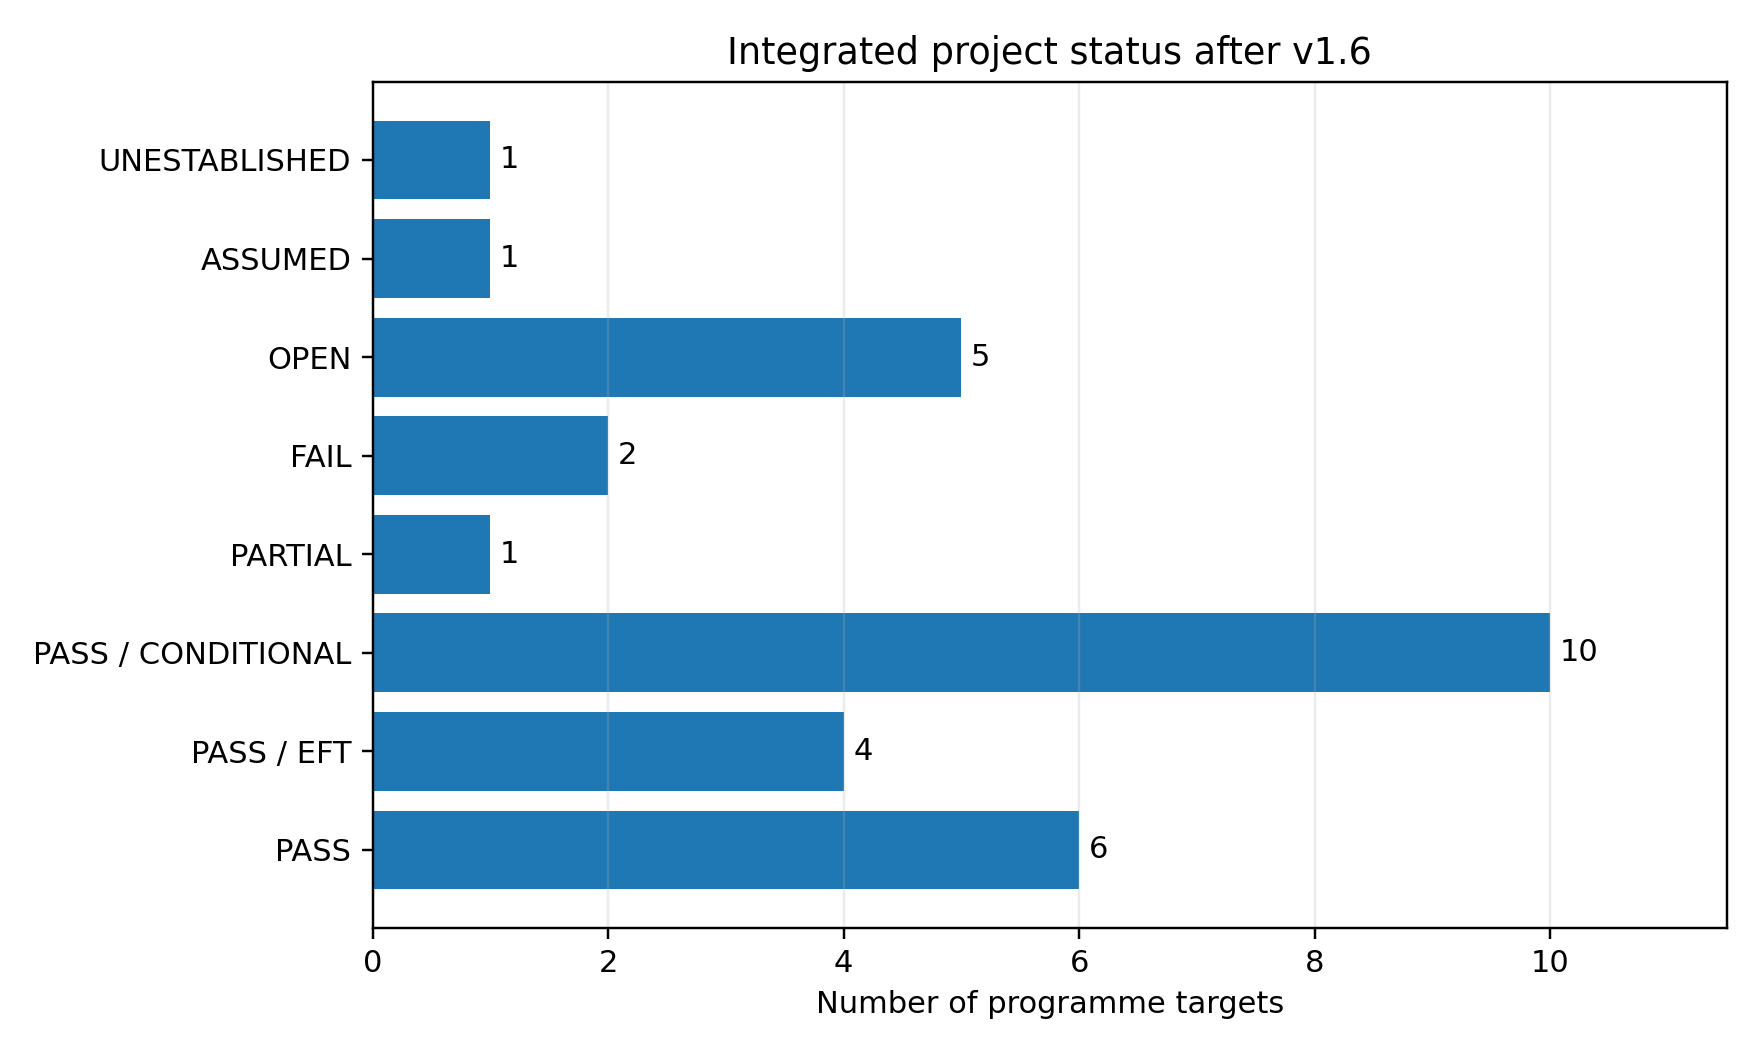
\includegraphics[width=0.86\textwidth,height=\textheight]{integrated_status_v1_6.png}
\caption{Integrated project status after v1.6.}
\end{figure}

The machine-readable matrix is supplied separately as
\texttt{integrated\_acceptance\_matrix\_v1\_6.csv}.

\section{References and overlap map}\label{references-and-overlap-map}

\begin{enumerate}
\def\labelenumi{\arabic{enumi}.}
\tightlist
\item
  Ehlers, Pirani and Schild, constructive foundations of spacetime
  geometry.
\item
  Fletcher, \emph{Light Clocks and the Clock Hypothesis}.
\item
  Menon, Linnemann and Read, \emph{Clocks and Chronogeometry}.
\item
  Damour and Donoghue, dilaton charges and equivalence-principle tests.
\item
  Chetyrkin, Kniehl and Steinhauser, QCD decoupling and low-energy
  theorems.
\item
  Das and Hook; Brzeminski et al., cyclic/discrete-Goldstone protection.
\item
  Arnold, Moore and Yaffe, leading-order effective kinetic theory.
\item
  Bodeker and Schroder, complete leading-order right-handed-electron
  equilibration.
\item
  Besak and Bodeker, complete leading-order ultrarelativistic
  right-handed-neutrino production.
\item
  Volovich, \emph{Gravitation and Spacetime: Emergent from Spinor
  Interactions - How?} (2026), which explicitly assigns geometric scale
  to massive-particle Compton clocks and Higgs breaking of conformal
  invariance.
\end{enumerate}

\section{Bottom line}\label{bottom-line}

The honest answer is:

\[
\boxed{
\begin{gathered}
\text{Yes, the project has produced work worth sharing.}\\
\text{Yes, some of it may be publishable and original in combination.}\\
\text{No, we have not yet established a new theory of time or gravity.}\\
\text{The next professional step is independent validation and paper separation, not more conceptual sprawl.}
\end{gathered}
}
\]

\end{document}
